\chapter{系统设计与实现}
本章介绍基于上述提出的各个模型所设计实现的一个基于知识图谱的IT运维辅助系统。实时运行的集群中存在着大量的组件与实时发生的事件,IT运维人员面对海量的信息需要花费大量时间和精力逐步查询分析多来源的繁杂数据。一个基于知识图谱的IT运维辅助系统可以有效地辅助运维人员,帮助其及时发现集群异常并预测可能出现的故障,从而大大降低了运维难度。本文设计实现的系统通过jaeger、prometheus、阿里云公开API等方式获取集群拓扑结构、微服务间拓扑结构、日志数据和指标时序数据,将集群实时运行状态可视化。随后,历史监测数据被按故障类型分组,经过事件因果关系挖掘模型构建了每种故障对应的组件-事件知识图谱。基于构建的组件-事件知识图谱,利用上文提出的表示学习模型和故障预测模型,本系统可以根据实时发生的事件序列预测可能会发生的故障,提醒运维人员及时采取应对措施。本章主要分为以下四部分来介绍系统:系统框架设计、数据获取、系统实现和功能展示。
\section{系统框架设计}
\subsection{系统框架}
本系统使用B/S架构,即浏览器发出请求,服务器给出响应的工作模式。整体架构分为模型(model)、视图(view)和控制器(control)三部分,即基于MVC模式解耦了系统各个模块。其中,模型在应用程序中负责处理数据和业务逻辑,即从数据库中读取数据后,根据业务逻辑处理数据;视图负责将数据显示给用户,视图显示的数据来自于模型根据业务逻辑处理后的数据;控制器则是从视图中读取数据,规范用户输入,发送数据给模型,完成了用户交互部分。另外,按照系统功能又可以把系统结构划分为数据层、业务逻辑层和交互层。图\ref{system-constructure}展示了这三层架构。

(1)数据层。本系统的数据层主要包含了日志数据、指标时序数据、集群组件拓扑和微服务间拓扑。这四类数据有不同的获取方式,具体获取方式在小节\ref{data-collect-way}进行了具体描述。

(2)业务逻辑层。业务逻辑层连接了数据层与交互层,包含了算法模型和业务逻辑。该层有多个模块协同实现系统功能,分为事件生成模块、组件拓扑生成、集群状态检测模块、事件因果判别模型、组件-事件知识图谱生成、故障预测模型。各个模块的协同工作实现了系统的核心共嗯那个,每个模块的具体功能在\ref{system-function}小节展开具体的介绍。
\begin{figure}[htbp]
    \centering
    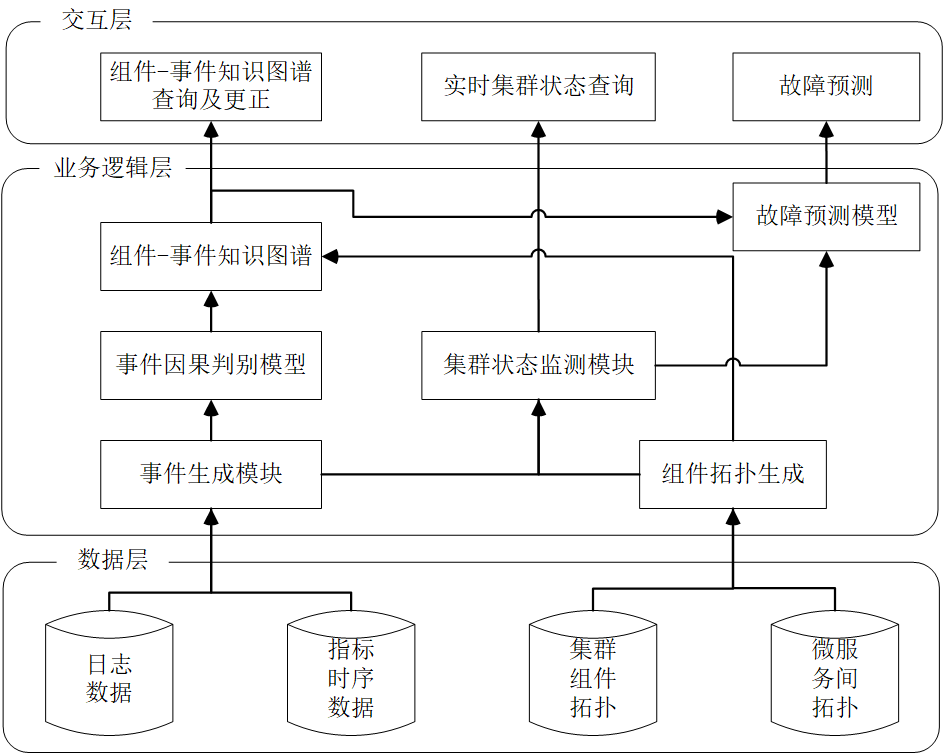
\includegraphics[width=0.8\textwidth]{system-constructure.png}
    \caption{IT运维辅助系统框架图\label{system-constructure}}
\end{figure}

(3)交互层。交互层将业务逻辑层数据可视化地直观展示在前端页面,并支持用户操作数据持久化到数据层。本系统交互层主要分为三部分:组件-事件知识图谱查询及更正、实时集群状态查询和故障预测结果展示。

\subsection{系统功能}\label{system-function}
系统功能已在图\ref{system-constructure}中业务逻辑层展示,分为:a.事件生成模块、b.组件拓扑生成模块、c.集群状态监测模块、d.事件因果判别模块、e.组件-事件知识图谱生成模块、f.故障预测模块。事件生成模块将多源异构数据统一转化为规范的事件类型数据。组件拓扑生成模块通过分析集群组件属性信息列表,利用其中表明了集群组件关系的字段生成了集群组件拓扑,而微服务间的拓扑则利用其实际工作时的访问关系生成。集群状态监测模块,则是将前两个模块数据,利用事件发生所在的组件位置连接起来,得到了可视化的集群运行状态图。事件因果关系判别模块会分析事件生成模块所产生事件间的因果关系。组件-事件知识图谱生成模块是从某类故障的历史数据中沉淀出包含组件依赖关系、组件事件产生关系和事件因果关系的该故障组件-事件知识图谱。故障预测模块基于集群状态监测模块所收集的事件序列,联合知识图谱预测未来可能发生的故障。下面具体介绍这些模块的功能:

(1)事件生成模块:该模块使用多线程调用阿里云公开API读取日志数据、指标时序数据。同样用多线程调用人工模板将数据转为事件类型数据。

(2)组件拓扑生成模块:内部使用数据库查询语句,快速获取集群组件与微服务连接关系,从而整合两部分拓扑构建组件拓扑图。

(3)集群状态监测模块:该模块负责汇总组件拓扑和事件信息,同时在交互页面点击组件时,该模块会返回组件属性信息和指标时序信息。

(4)事件因果判别模块:该模块使用判别模型对事件候选关系二分类,类别为有无因果关系。在判别关系时,输入为两个事件特征向量,输出为有因果关系的概率。

(5)组件-事件知识图谱生成模块:知识图谱的生成即是从历史数据中沉淀知识的过程。本模块收集历史数据,包括事件因果关系对和相应组件拓扑图,然后按故障类型分组历史数据,依次合并每组数据,即可得到对应故障类型的组件-事件知识图谱。

(6)故障预测模块:该模块中,输入为集群状态监测模块所收集的发生在组件拓扑上以时间顺序排列的事件序列,另外组件-事件知识图谱也会被输入到该模块中,最后按照相似度降序输出候选故障类型即可。


\section{数据获取}\label{data-collect-way}
系统需要从多个源头获取多种类别的数据。系统需要获取的数据共有4种,包括集群拓扑结构、微服务拓扑结构、日志数据、指标时序数据。下面分为四部分分别介绍这四种数据具体的获取方式。
\subsection{集群拓扑结构}
第一部分为集群拓扑结构数据的获取,分为以下步骤:

(1)系统开发时,引入阿里云提供的SDK核心库和组件的Maven项目依赖。

(2)编写多线程代码调用不同组件的数据请求方法并设置参数,再保存方法返回的Json数据。如调用方法$DescribeImagesRequest(.)$,设置要查询的镜像类型$setImageOwnerAlias(.)$,就会返回对应镜像的Json格式的基本信息。

(3)分析返回的Json数据,读取指定字段值。
返回的Json数据不同字段包含着不同类型的信息,如字段$ ImageId: freebsd\_11\_02\_64\_30G\_alibase\_20190722.vhd$表明了镜像的唯一标识符;$OSNameEn: FreeBSD  11.2 64 bit$表明了系统名称;$VpcId:vpc—2zeuphj08tt7q3brd****$表明了ECS所在VPC的唯一标识符。

(4)按获取的字段信息构建实体属性列表,和组件间关联拓扑。

\subsection{微服务拓扑结构}
第二部分为微服务拓扑结构的获取。微服务依赖关系虽然在分布式应用的代码逻辑中已清晰规定,但应用的代码属于机密信息且阅读代码时耗过大。为了无需了解应用代码逻辑就可以获取微服务间访问拓扑关系,本系统选用开源Jaeger实时监控并收集微服务间的访问信息。
\begin{figure}[htbp]
    \centering
    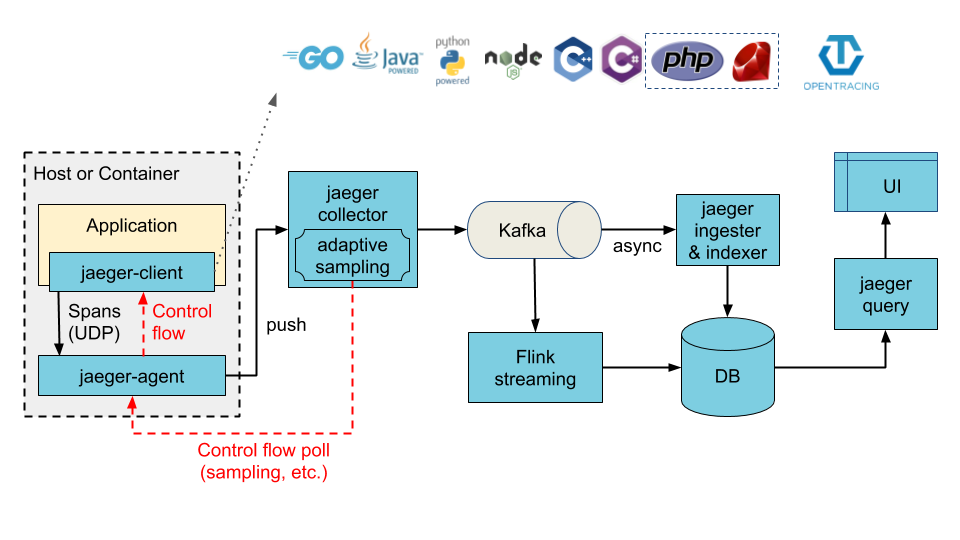
\includegraphics[width=0.8\textwidth]{jaeger-system-constructure.png}
    \caption{Jaeger架构图\label{jaeger-system-constructure}}
\end{figure}

Jaeger架构图如图\ref{jaeger-system-constructure}所示,可见包含以下几个部分:

(1)\textbf{jaeger client libraries。}jaeger客户端是基于OpenTracing API的特定语言实现的,可通过与OpenTracing集成的各种现有开源框架来检测应用程序以进行分布式跟踪。它会以较小的开销始终在后台开启,不断采样Span并异步传输到Jaeger Agents。采样策略默认为随机采样0.1\%。

(2)\textbf{jaeger agents。}Agent是网络守护程序,负责侦听通过UDP传输的Span,并分批次将Span发送给Collector。另外,它作为一种基础结构组件会被部署到所有主机。

(3)\textbf{Collector。}collector在接收到Agent传来的Span后,会验证跟踪并为这些Span建立索引,并最终存储起来。Jaeger使用的存储设备是可插拔的,目前支持Cassandra、Elasticsearch和Kafka。

(4)\textbf{Query。}Query是一项从存储中检索微服务依赖信息,并用UI显示的服务。

(5)\textbf{Ingester。}Ingester负责提供从Kafka读取数据并写入其他存储后端的服务。
\begin{figure}[htbp]
    \centering
    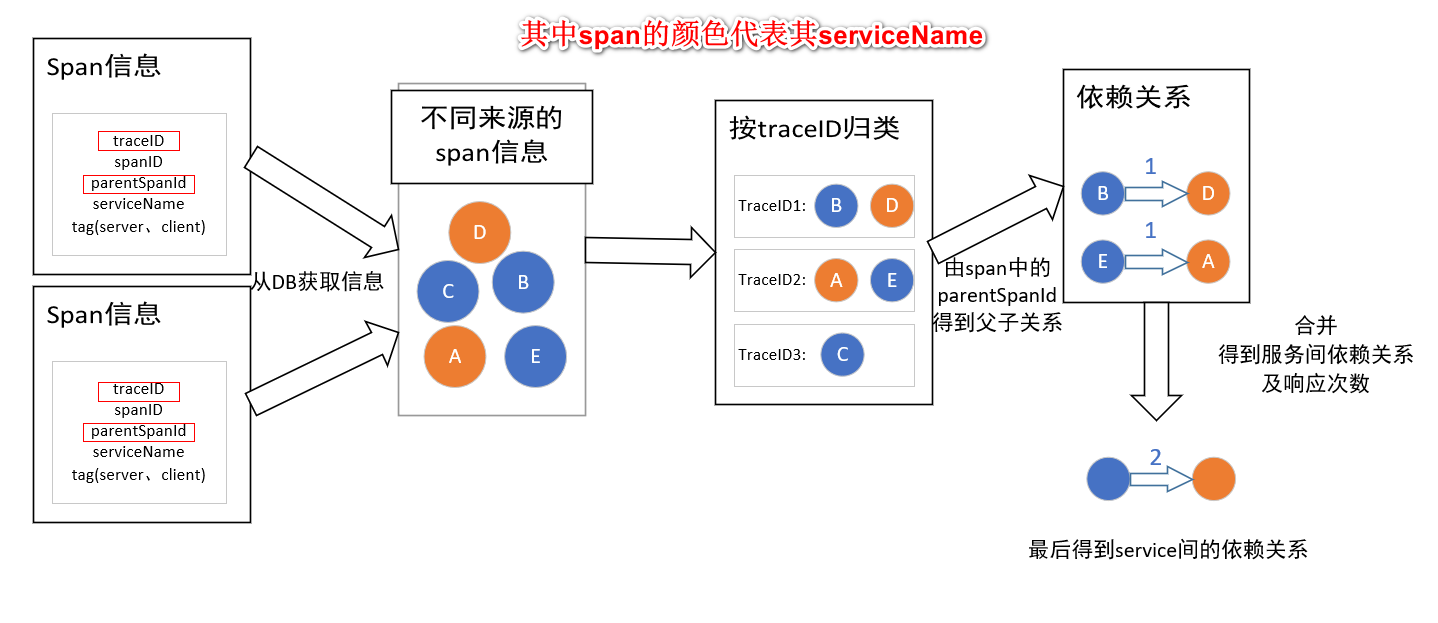
\includegraphics[width=0.8\textwidth]{tracing-generate.png}
    \caption{微服务间依赖图生成流程\label{tracing-generate}}
\end{figure}

其中,一个Span对应一条微服务被调用的记录,其记录了对应微服务被标识符为parentSpanID的Span中的微服务调用了一次。一个Trace对应了分布式应用完成一个业务请求时,微服务之间的一条请求链路。而微服务拓扑图的生成是由Flink Streaming块完成的。其整体流程如图\ref{tracing-generate}所示。分为以下步骤:

(1)获取Span数据。从Kafka中读取一个时间段内所有来源的Span。

(2)分组Span数据。将所有Span按照traceID分组,这样就获得了traceID到Span集合的映射关系。

(3)分析同组Span间依赖关系。遍历每个Span对应的ParentSpanID,得到Span之间的父子依赖关系。

(4)生成微服务间依赖关系。根据Span中serviceName信息,将Span间依赖关系映射为微服务间依赖关系。

(5)微服务间拓扑图生成。将不同Trace中微服务间依赖关系整合规约,生成微服务拓扑图结构。

\subsection{日志数据}
第三部分为日志数据的收集。日志数据的收集分为以下步骤:

(1)日志数据采集。阿里云日志服务(Log Service, SLS)提供了数据投递、查询、消费和采集等功能,可以高效的处理海量日志。在阿里云日志服务中创建Logstore,选择DockerIO、k8s日志等作为数据源,日志服务就会实时将数据汇总收集起来。
\begin{figure}[htbp]
    \centering
    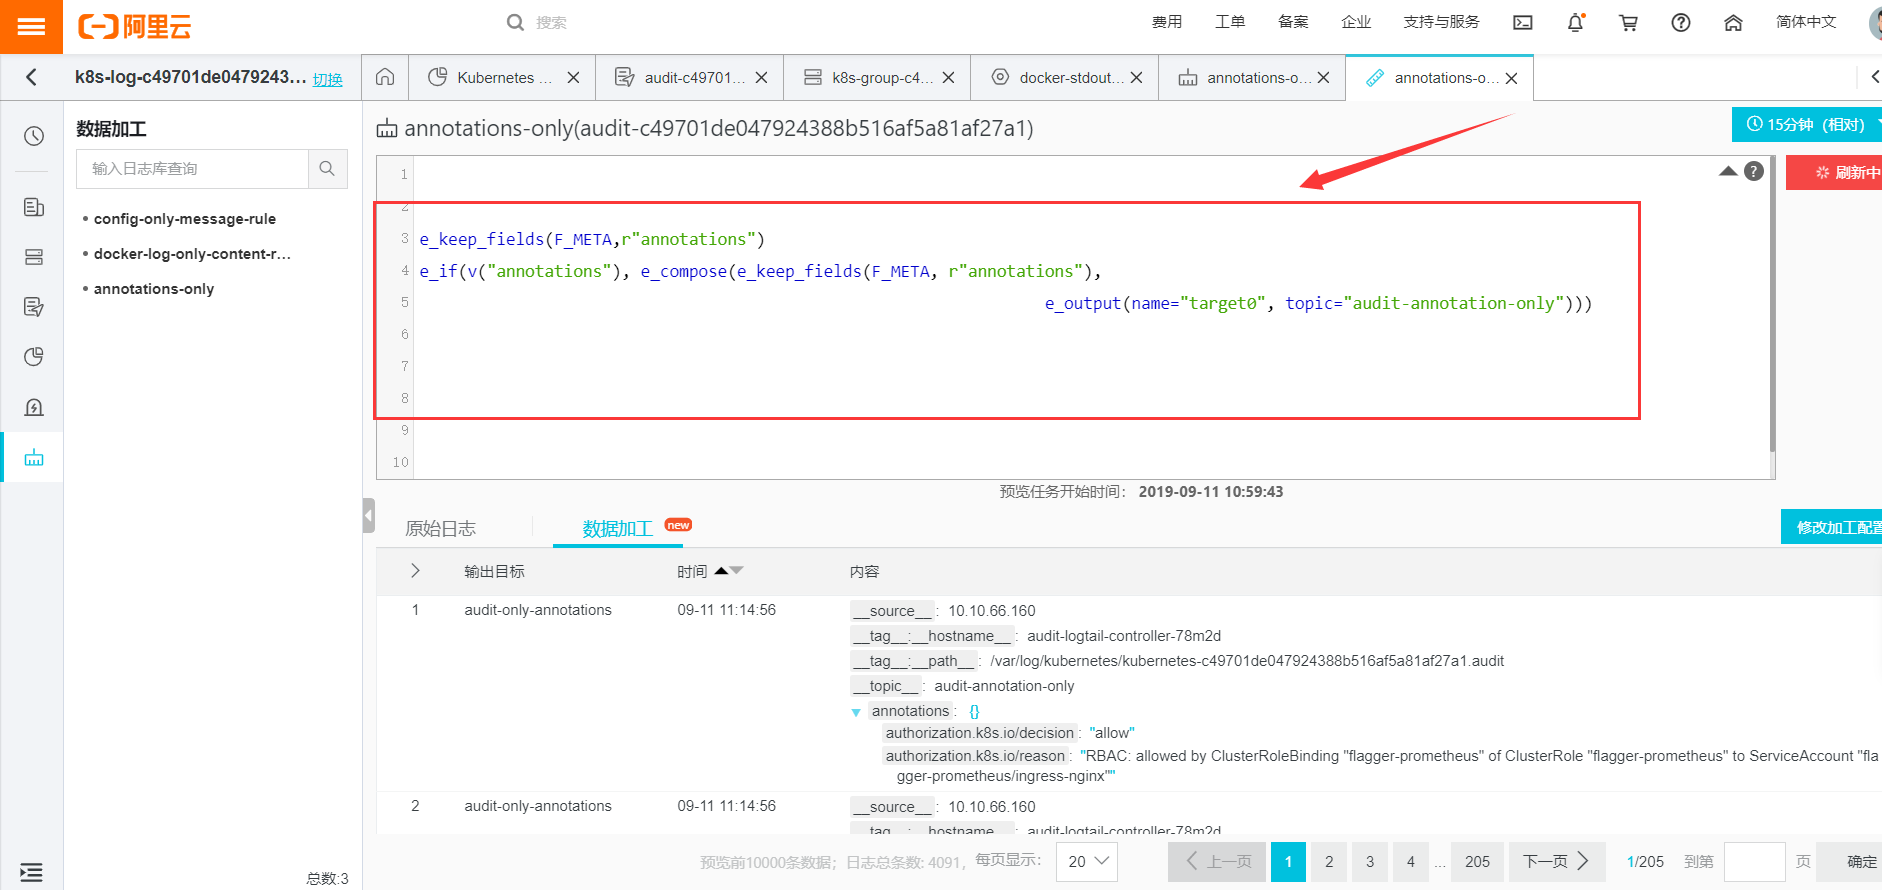
\includegraphics[width=0.8\textwidth]{data-process.png}
    \caption{数据加工指令\label{data-process}}
\end{figure}

(2)日志数据加工。由于原始日志数据包含了很多无效信息,上一步得到的原始日志需要进一步加工处理只保留有效字段信息。加工过程直接使用日志服务的数据加工功能,编写加工命令(如图\ref{data-process}所示)选取保留的字段,并传输到新的Logstore中即可。图\ref{sls-audit-cluster}为数据加工实例,该例中只保留了audit数据中的annotation字段。

\begin{figure}[htbp]
    \centering
    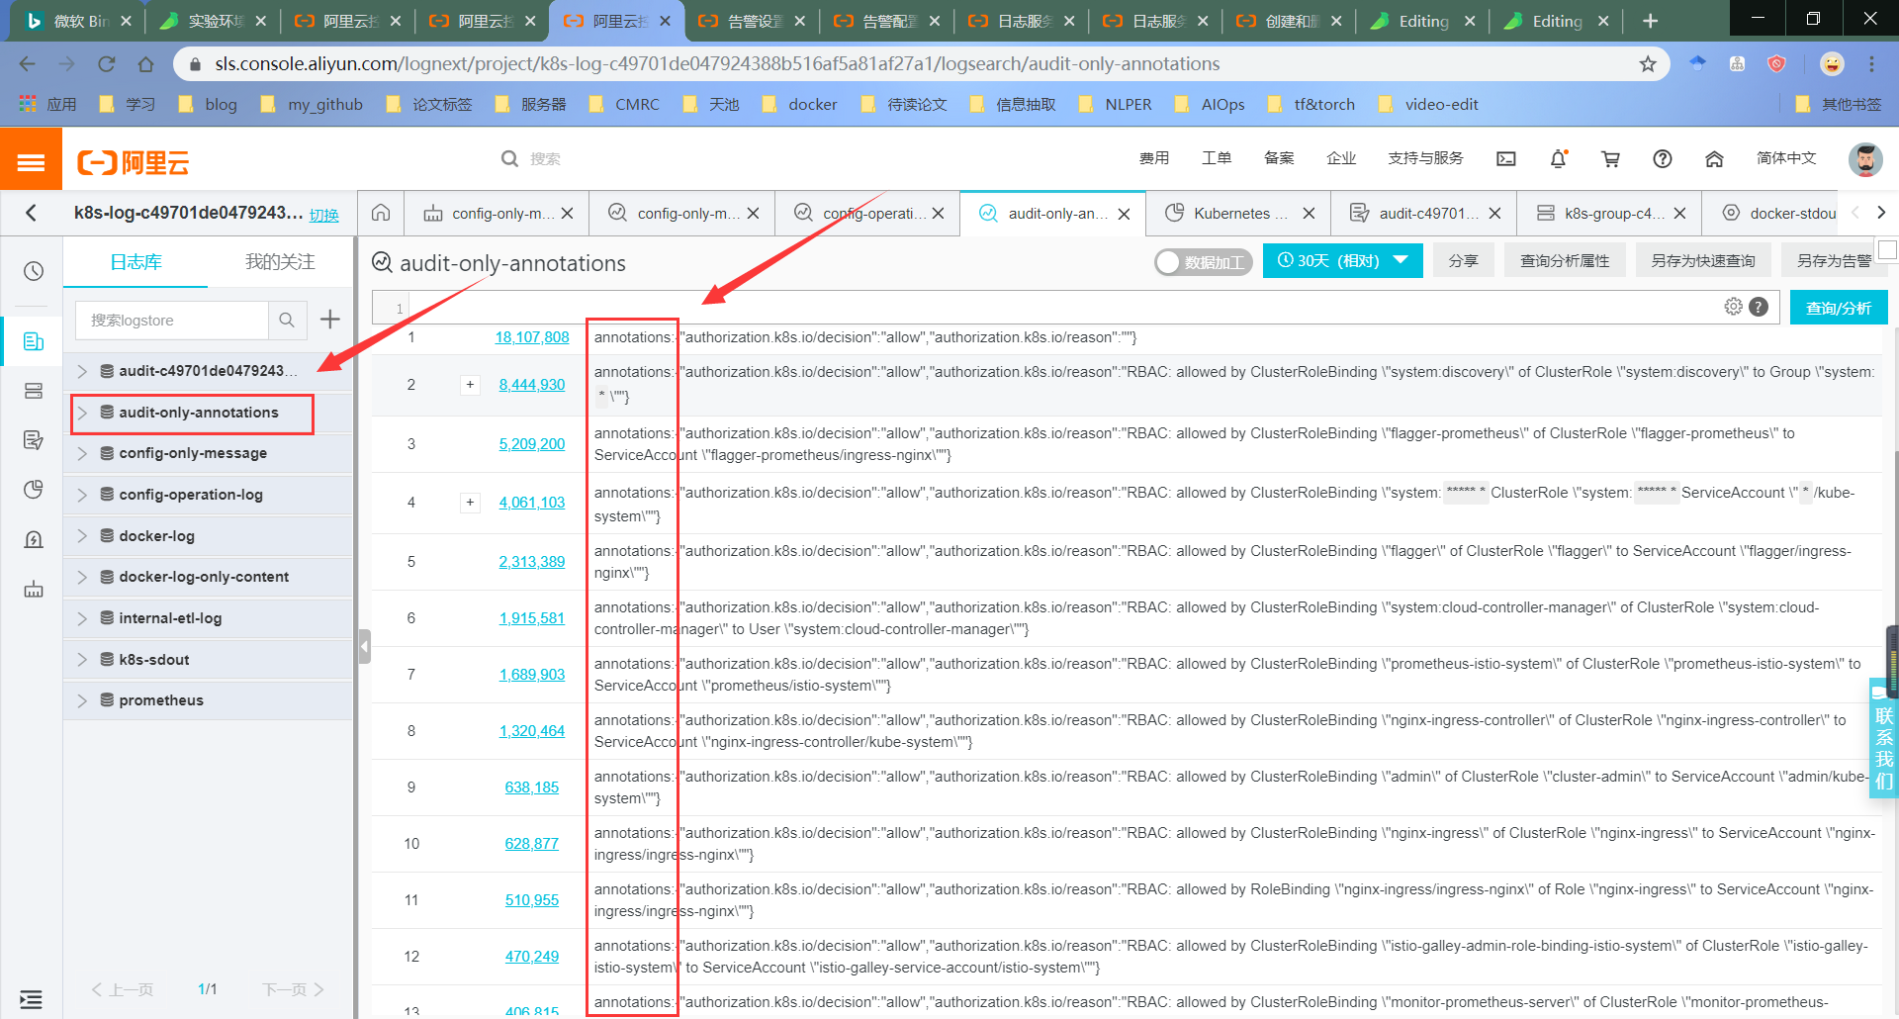
\includegraphics[width=0.8\textwidth]{sls-audit-cluster.png}
    \caption{数据加工结果实例\label{sls-audit-cluster}}
\end{figure}

(3)公开API请求日志数据。经过上述步骤,日志数据被存储在日志服务各个Logstore中。当系统需要获取某段时间日志数据时,系统直接使用公开API并设置参数请求即可。如使用函数$PullLogsRequest(project, logStore, shardId, logNum, cursor);$并设置所要消费的project、LogStore和每次读取日志数量logNum等参数,就会返回符合参数约束的日志数据。

\subsection{指标时序数据}
第四部分为获取指标时序数据。指标时序数据均为曲线类的数据,在存储形式上,均为一组时间戳到值的映射关系集合。

(1)指标时序数据检测。在分布式集群中,多种组件都会有指标时序数据,且每个组件上会有不同种类的指标时序数据,如cpu、内存、磁盘吞吐率等。系统选用了prometheus进行实时的监测。

(2)指标时序数据长期存储。由于prometheus监测得到的指标时序数据不能长期存储(一般只保留14天),系统为了长期存储选择将数据导入日志服务。图\ref{metric-prometheus}展示了指标时序数据导入日志服务后的结果,可见每条数据都对应着一个时间戳到值的映射关系。

\begin{figure}[htbp]
    \centering
    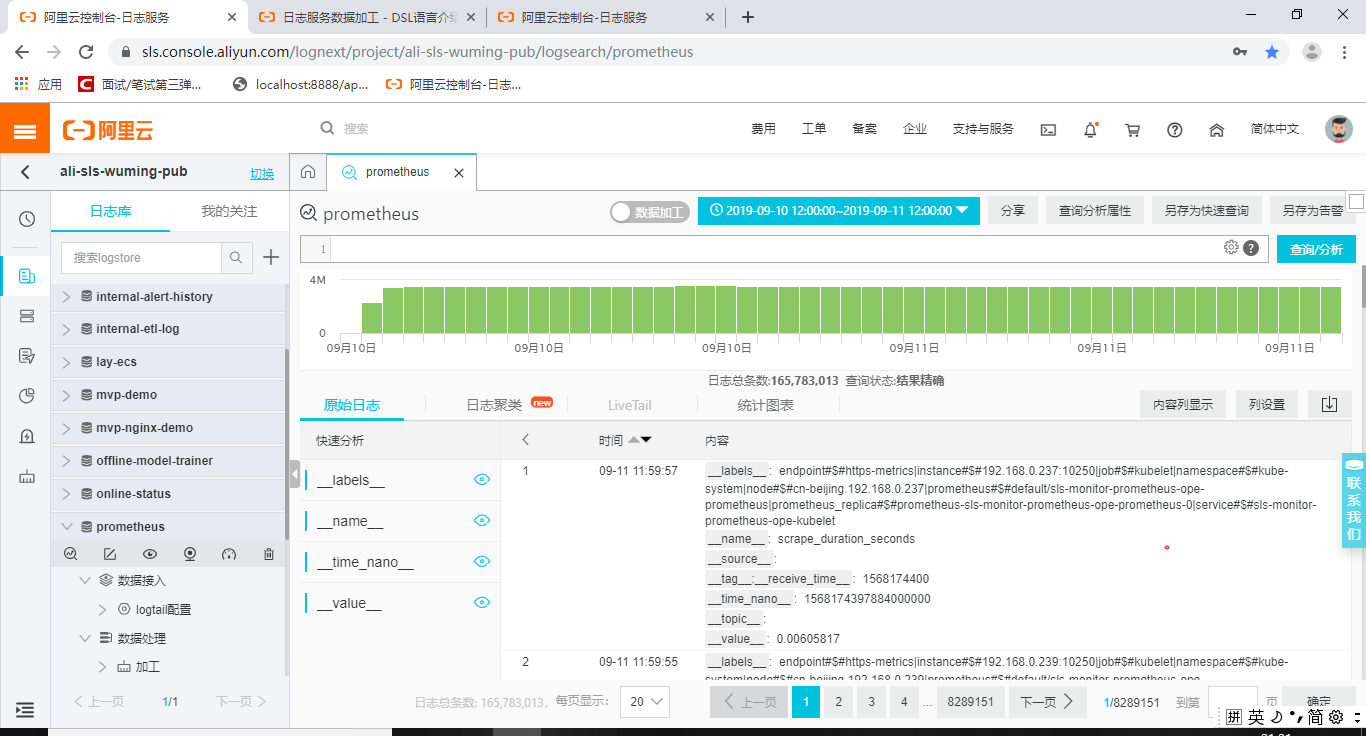
\includegraphics[width=0.8\textwidth]{metric-prometheus.png}
    \caption{数据加工结果实例\label{metric-prometheus}}
\end{figure}
(3)公开API获取指标时序数据。将数据长期存储入日志服务平台后,系统可采用请求日志的API来请求获取指标时序数据。

\section{系统实现和功能展示}
\subsection{系统实现}
本文所设计实现的IT运维辅助系统采用了B/S架构,用户可以通过web端访问系统。开发本系统的环境为:11th Gen Intel(R) Core(TM) i5-11300H CPU 3.11GHz,16G内存;操作系统为64位Windows 10,系统开发工具为Intellij IDEA,开发语言为Java, jdk版本为1.8.0.60。整个IT运维辅助系统使用Spring Boot开发后台,Vue.js编写前端,Neo4j存储图数据,从而实现了MVC框架。此外,根据系统需求,选用了一些开源组件和服务,包括Jaeger、Flink、Kafka、阿里云日志服务和Echarts等,相关技术如图\ref{system-technology}所示。下面对所使用到的技术展开了具体介绍:

(1)Spring Boot:Spring框架为基于Java的企业应用程序提供了一个全面的编程和配置模型。它通过为应用程序提供基础的支持,使得团队可以关注应用程序层次的业务逻辑,而不必过于关注特定的部署环境。SpringBoot为Java开发人员提供了一个很好的平台,便于开发人员开发一个独立的、生产级的Spring应用程序。其优势包括易于理解和开发spring应用程序、提高生产力、缩短了开发时间。本系统使用SpringBoot完成了数据读取以及主要的业务逻辑功能模块。

(2)Neo4j:neo4j 与传统关系型数据库不同,是一个高性能的 nosql 的图数据库,使用图结构组织存储结构化数据。在关系型数据库中,一旦数据表的结构被确定,表中列的修改成本较大,而对于图数据库,记录的属性可以方便的添加和删除。另外,图数据库提供了图路径查询等功能,在本系统中,需要根据组件-事件拓扑关系生成路径,因此,系统使用neo4j 存储组件-事件的拓扑关系。

(3)Jaeger:Jaeger 是一个分布式跟踪系统,由Uber技术公司作为开源项目发布。它被用于监视和排除基于微服务的分布式系统的故障,包括以下方式分布式上下文传播、分布式事务监控、根本原因分析、服务依赖性分析和性能优化。本系统使用jaeger监测并获取了分布式应用各个微服务之间的依赖拓扑。

(4)Kafka:Kafka是一个分布式系统,由通过高性能TCP网络协议进行通信的服务器和客户机组成。它可以部署在本地和云环境中的裸机硬件、虚拟机和容器上。它主要拥有三项功能,分别为a.发布(写入)和订阅(读取)事件流,包括从其他系统连续导入/导出数据;b.持久可靠地存储事件流;c.当事件发生或追溯时处理事件流。所有这些功能都是以分布式、高度可扩展、弹性、容错和安全的方式提供的。在本系统中,Kafka被用于缓冲从集群各个组件收集来的实时数据。

(5)阿里云日志服务:日志服务(SLS)是云原生观测分析平台,为Log/Metric/Trace等数据提供了大规模、低成本、实时平台化服务。一站式提供数据采集、加工、分析、告警可视化与投递功能,全面提升研发、运维、运营和安全等场景数字化能力。阿里云日志服务是本系统收集、分析日志的重要工具。

(6)Promethues:Prometheus是一个开源的系统监控和警报工具包。普罗米修斯使用度量名称和键/值对识别时间序列数据的多维数据模型。普罗米修斯可以很好地记录任何纯数字时间序列。它既适用于以机器为中心的监视,也适用于高度动态的面向服务体系结构的监视。在微服务的世界中,它对多维数据收集和查询的支持是一个特别的优势。本系统即是使用普罗米修斯获取各个组件上各种时序数据。

(7)Vue.js:Vue.js是一个用于构建交互式web界面的库。它主要关注MVVM模式的ViewModel层,并通过双向数据绑定连接视图和模型。它是一个用于构建用户界面的渐进式框架。与其他单片框架不同,Vue.js从一开始就被设计成可增量的。核心库只关注于视图层,并且易于获取并与其他库或现有项目集成。另一方面,当与现代工具和支持库结合使用时,Vue.js也完全能够为复杂的单页应用程序提供动力。本文使用Vue.js开发了系统前端架构。

(8)Echarts:Echarts是一个开源的JavaScript可视化工具,可以在PC和移动设备上流畅地运行。它与大多数现代网络浏览器兼容,例如IE8/9/10/11、Chrome、Firefox、Safari等等。ECharts依靠ZRender(一个图形渲染引擎)来创建直观、交互式和高度可定制的图表。本系统在向用户展示数据时,使用Echarts设计了各种图标。

\begin{figure}[htbp]
    \centering
    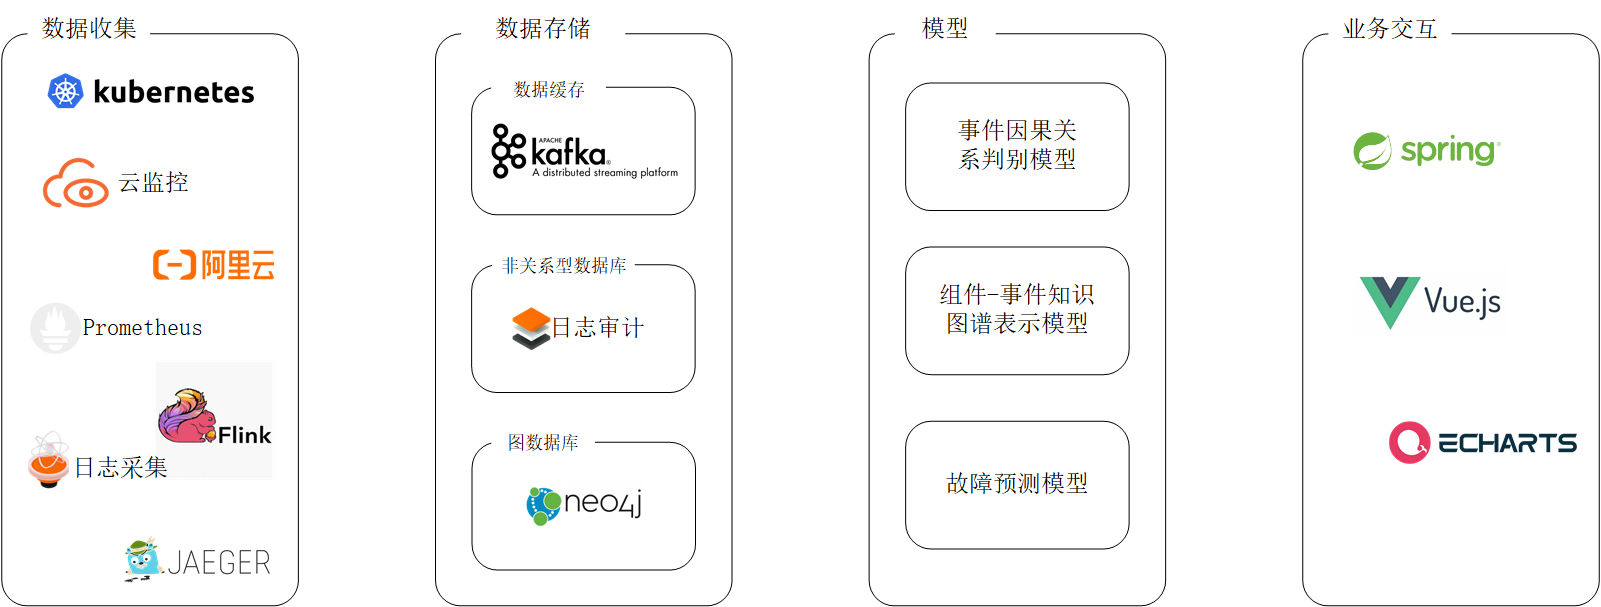
\includegraphics[width=0.8\textwidth]{system-technology.png}
    \caption{IT运维辅助系统相关技术\label{system-technology}}
\end{figure}

在模型方面,系统共使用了事件因果判别模型、组件-事件知识图谱表示学习模型、基于知识图谱和时序数据的故障预测模型。事件因果判别模型,输入事件对特征向量,输出事件对间存在因果关系概率。组件-事件知识图谱的表示学习模型在训练时,输入三元组及其背景拓扑结构,以三元组是否成立以及实体类别为损失函数训练模型。将训练完成的表示学习模型作为嵌入层,将故障类型对应的组件-事件知识图谱输入嵌入层,将事件序列输入双向记忆网络,最后以两者相似度降序排列输出预测故障类型。基于以上模型,本系统可以实时展示集群各种维度信息状态、提前预测可能会出现的故障。

\subsection{功能展示}
下面分为各部分展示本系统所实现的功能:
(1)组件信息查看。图\ref{component-detail-info}展示了将鼠标悬停在组件上,就会在右上方显示该组件属性信息列表。图\ref{search-component-metric-info}展示了左键点击组件时,会在右侧抽屉弹出该组件的各种指标时序信息。
\begin{figure}[htbp]
    \centering
    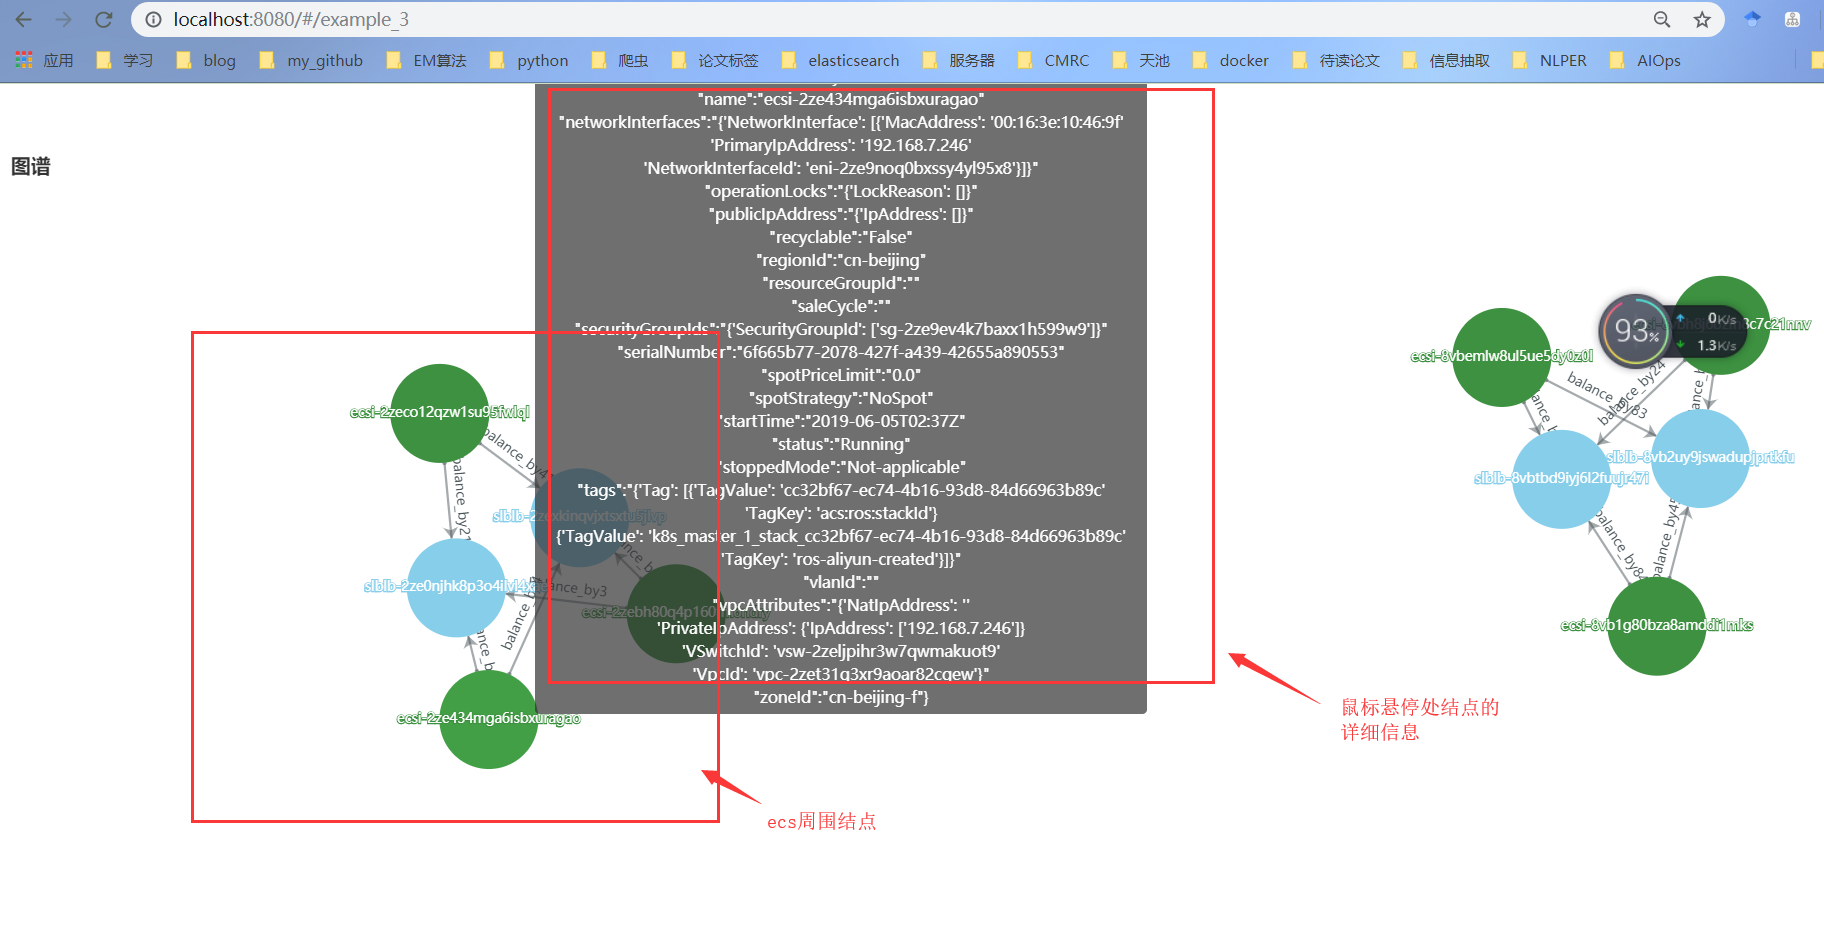
\includegraphics[width=0.8\textwidth]{component-detail-info.png}
    \caption{组件属性信息\label{component-detail-info}}
\end{figure}
\begin{figure}[htbp]
    \centering
    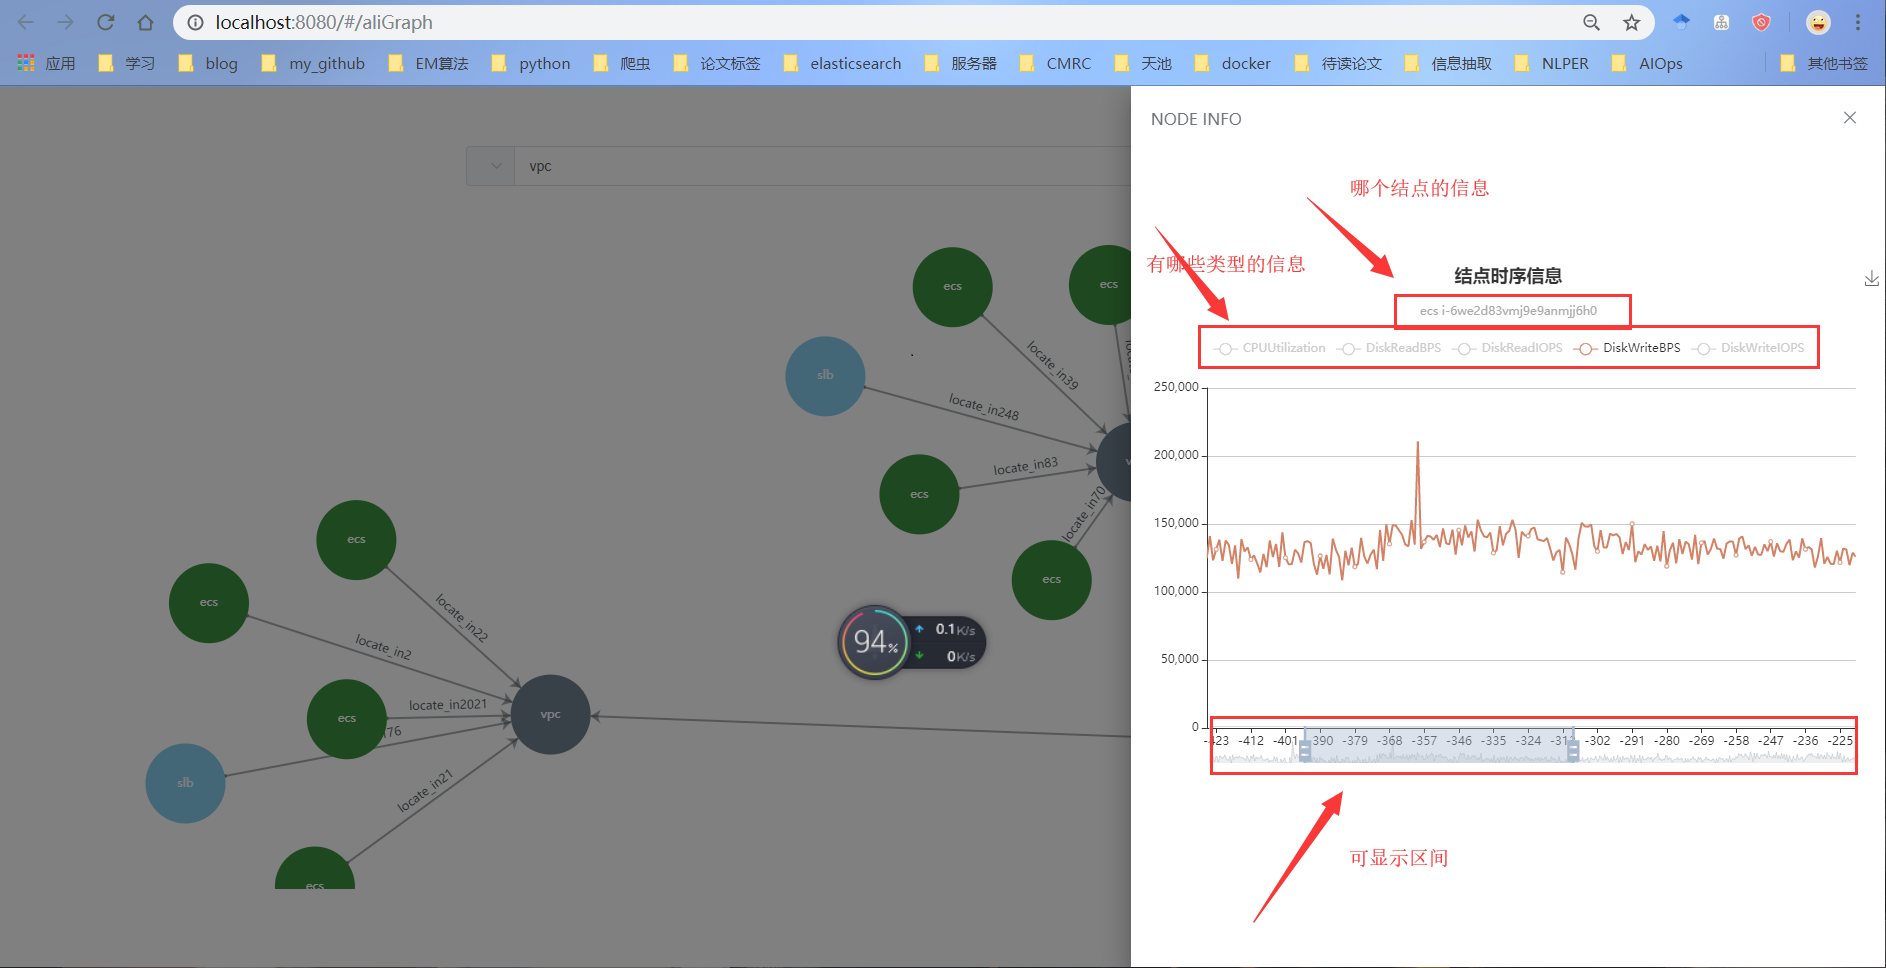
\includegraphics[width=0.8\textwidth]{search-component-metric-info.png}
    \caption{组件指标时序信息\label{search-component-metric-info}}
\end{figure}

(2)条件搜索。图\ref{search-component-path}显示了搜索符合 vpc-slb-ecs 类型关系的所有拓扑路径。图\ref{search-detail-component}显示了搜索指定id的vpc组件及其周边结点。

\begin{figure}[htbp]
    \centering
    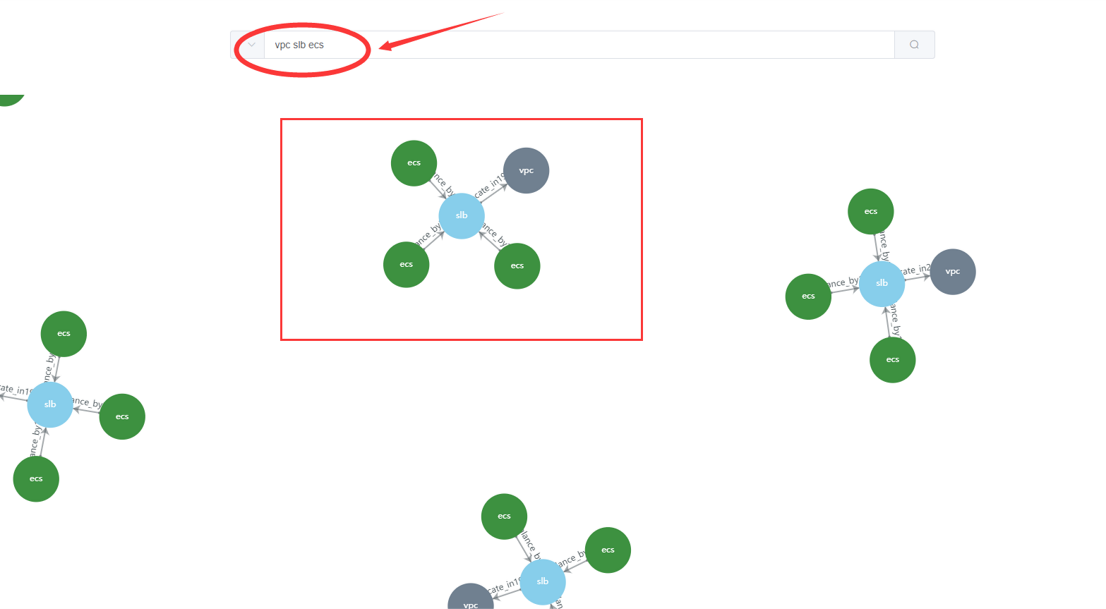
\includegraphics[width=0.8\textwidth]{search-component-path.png}
    \caption{搜索指定路径\label{search-component-path}}
\end{figure}

\begin{figure}[htbp]
    \centering
    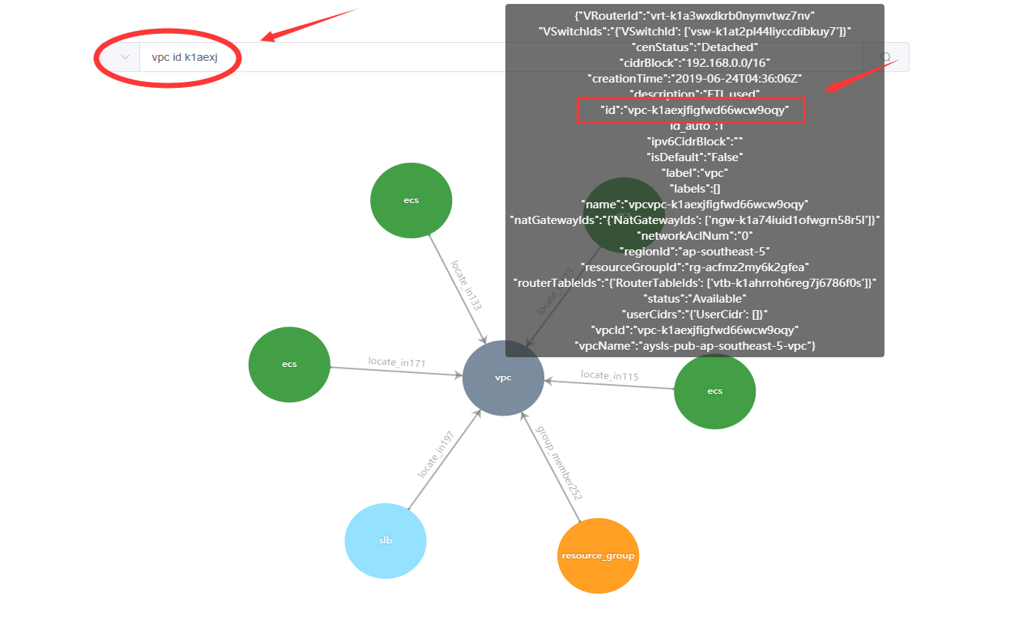
\includegraphics[width=0.8\textwidth]{search-detail-component.png}
    \caption{搜索指定结点\label{search-detail-component}}
\end{figure}

(3)查看事件知识图谱。图\ref{}展示了故障代号为f3的组件-事件知识图谱。在最上层为事件层,中间为微服务层,下层为集群组件层。

\begin{figure}[htbp]
    \centering
    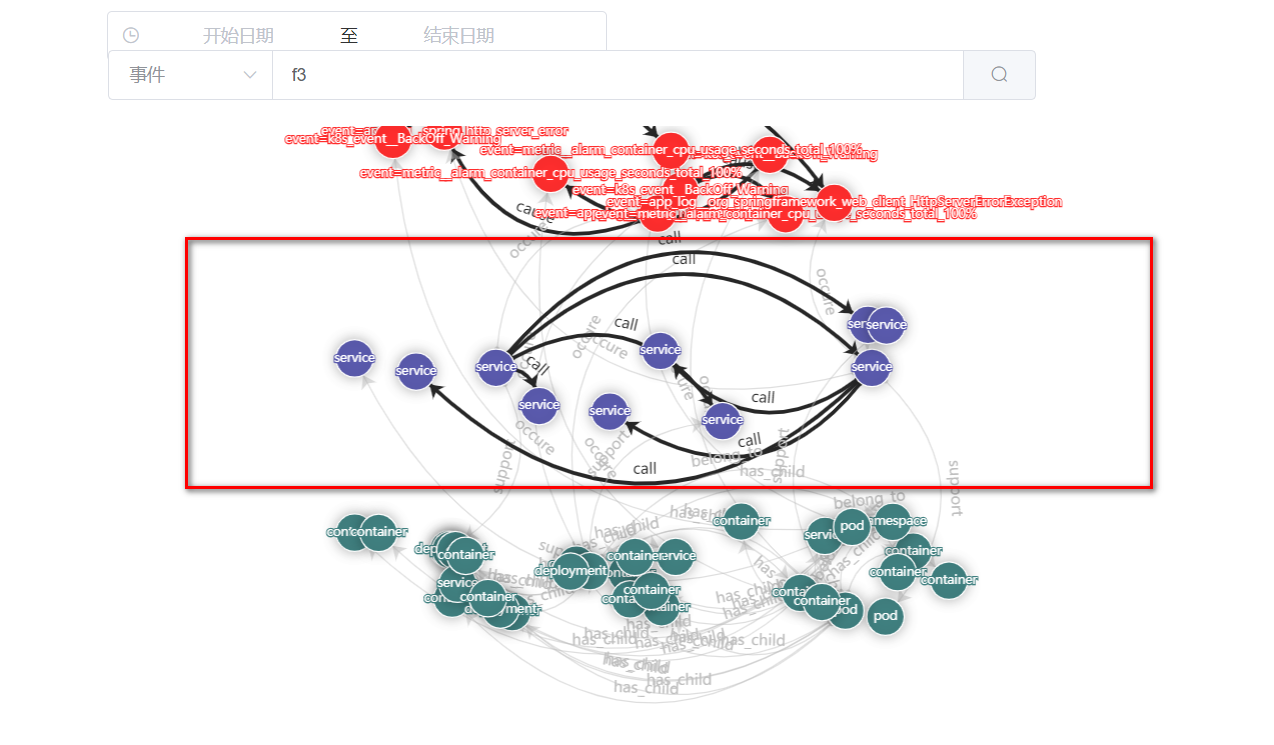
\includegraphics[width=0.8\textwidth]{device-service-event.png}
    \caption{查看f3故障类型的组件-事件知识图谱\label{device-service-event}}
\end{figure}

(4)故障预测。

\section{本章小结}
本章介绍了基于知识图谱的IT运维辅助系统,包括系统架构、系统功能和数据收集方式,并给出了系统功能的
展示案例。